%
% File acl2016.tex
%
%% Based on the style files for ACL-2015, with some improvements
%%  taken from the NAACL-2016 style
%% Based on the style files for ACL-2014, which were, in turn,
%% Based on the style files for ACL-2013, which were, in turn,
%% Based on the style files for ACL-2012, which were, in turn,
%% based on the style files for ACL-2011, which were, in turn, 
%% based on the style files for ACL-2010, which were, in turn, 
%% based on the style files for ACL-IJCNLP-2009, which were, in turn,
%% based on the style files for EACL-2009 and IJCNLP-2008...

%% Based on the style files for EACL 2006 by 
%%e.agirre@ehu.es or Sergi.Balari@uab.es
%% and that of ACL 08 by Joakim Nivre and Noah Smith

\documentclass[11pt]{article}
\usepackage{acl2016}
\usepackage{times}
\usepackage{url}
\usepackage{latexsym}
\usepackage{graphicx}

\aclfinalcopy % Uncomment this line for the final submission
%\def\aclpaperid{***} %  Enter the acl Paper ID here

%\setlength\titlebox{5cm}
% You can expand the titlebox if you need extra space
% to show all the authors. Please do not make the titlebox
% smaller than 5cm (the original size); we will check this
% in the camera-ready version and ask you to change it back.

\newcommand\BibTeX{B{\sc ib}\TeX}

\title{Caption Generation from Localized Image Labels}

  \author{Divya Sree Korimi \\
  Arizona State University \\
  Tempe, AZ, USA\\
  {\tt dkorimi@asu.edu} \\\And
  Adam Chmurzynski \\
  Arizona State University \\
  Tempe, AZ, USA\\
  {\tt achmurzy@asu.edu}  \\\And
	Nitesh Thali \\
 Arizona State University \\
  Tempe, AZ, USA\\
  {\tt nthali@asu.edu} \\}
  
\date{}
\begin{document}
\maketitle
\section*{\centering {Problem Statement }}
%\section{Problem Statement}
Here we propose to use labeled image data to generate natural language captions of an arbitrary photograph. Image labels will be provided by a dense-captioning algorithm [1] which locates salient features in an image and generates descriptive phrases localized by bounding boxes in the image space. Our approach will weight the most important descriptive phrases by confidence scores associated with each phrase from the dense-captioning algorithm, as well as a saliency metric from computer vision [2]. Our generative model will be based on auto-encoders trained on human-annotated image captions from the Visual Genome dataset and dense-captioned phrases. The auto-encoder will ultimately be able to output a caption given a set of salient phrases describing an image by learning phrase embedding from training data.  

\section{Motivation}
Vast amounts of image data exist with varying amounts of annotation from human or machine labeling and tagging. Humans may have a hard time understanding a photograph from a bag of words or phrases that define most labeling schemes. Instead, systems which create natural language sentences clearly describing a photograph may help users of applications more easily find content of a certain kind. Software able to generate a complete natural language description of a photograph may help create robust summarization systems for decision-makers or generate content for media companies online. Search performance on images may increase if natural language descriptions of pictures are included to more closely match user queries. 


\section{Current Adapted Method}
\subsection{Phrase Generation using DenseCap}
In the first step we have generated phrases from an image using DenseCap Software [3]. DenseCap provides a deep convolutional neural network trained in an end to end fashion on Visual Gnome dataset. We have run the model on new images available at MS-COCO (2014 Training Images) [4]. The MS-COCO dataset provides image caption annotations which are used to store image captions. Each annotation is represented by fields such as image\_id and caption, where each image consists of at least 5 captions.
\subsection{Ranking the Phrases}
Next, We are feeding the most important phrases to our RNN network instead of inputting all the phrases generated by DenseCap. In order to rank, we used the saliency algorithm [2] to determine which are the important phrases for an Image. The output of DenseCap is a JSON string containing phrases and bounding boxes along with importance scores. The bounding boxes are given as xy coordinate of upper left corner along with width and height.
\subsection{Training RNN model}
The Recurrent Neural Network (RNN) works by encoding the variable length input into a fixed dimensional vector, and uses this representation to “decode” it to the desired output sentence. We aim at maximizing the probability of generating correct caption given the image phrases and the model. To overcome the problem of vanishing gradient in RNN, we are using Long Short Term Memory Networks called LSTMs nets which are special kind of RNN capable of learning Long Term Dependencies. We will be feeding the salient phrases obtained from previous step to this RNN network to generate the desired caption.

\section{Justification for Current Adapted Method}
In our project we have used Recurrent Neural Nets (RNN) to generate captions as it is the state-of-the-art sequence generation method. While we compare with other methods such as feed-forward network, RNN proves to be much better, as in feed forward networks we shall have to choose the length of your input beforehand, and you will not be able to learn functions that depends on the inputs happening long time ago. You can solve this problem by having a RNN, that can theoretically, store information from arbitrarily long time ago, in its context layer.

On the other hand we have systems like And-Or Graphs or logic systems, which are further converted to natural language via rule-based systems. Such systems are heavily hand-designed, relatively brittle and have been demonstrated only on limited domains, e.g. traffic scenes or sports. In our model, with RNN we can overcome this overhead as we combine deep convolutional nets (from DenseCap) for phrase generation with recurrent networks for sequence modeling to create a single network that generates descriptions of images.
 
In here we have used a more powerful RNN model, and provide the phrase input to it directly, which makes it possible for the RNN to keep track of the words that have been explained by the text. As a result of these seemingly insignificant differences, our system achieves substantially better results when compared with others.

\section{Current Experiments and Results}
Our current architecture is depicted in Figure 1. We currently use a single layer of n hidden LSTM cells to generate sequences. Future experiments will involve varying the number of LSTM layers and the number of cells per layer. Our current architecture is somewhat arbitrary as we work to implement the entire pipeline. 
We represent training data as a 3D tensor of dimension (phraseCount, phraseLength, lexiconSize). Each of these represents parameters we intend to vary in future experiments. The first two are currently arbitrarily set to 5, and the lexiconSize is determined from the set of captions input from MS-COCO. The last dimension is used to represent words as 'one-hot' vectors, which are sparse boolean masks representing each word as a unique bit in a vector of length lexiconSize. 
Our output layer is currently under construction. We have successfully completed training sessions for a single image using a cross-entropy cost function for a truncated caption of length phraseLength. This is mostly due to the need for matching dimensions in input phrases and output captions; however, this is not ideal and does not accurately address our problem. Currently, we are attempting to create a sequence generation procedure using the trained network to generate captions for comparison to training captions. Using METEOR and BLEU, two machine translation accuracy metrics, we can compare two sequences independent of length. 
Future experiments will focus on two areas: input preprocessing to determine phrases the network is trained with, and varying network architecture and gradient descent methods to identify different caption-generation behaviors. 
The first area will be addressed by implementing new saliency metrics for determining the importance of phrases. Our current implementation naively relies on confidence scores associated with the dense captioning software.
The second area will include changing input format for different word representations. Specifically, the “one-hot” vectorization scheme does not permit a wide lexicon or account for realistic associations between similar words where training and test vocabulary may differ slightly. We will implement the Google word2vec framework for word representation. Additionally, our input format does not permit training on phrases of variable length. Dense cap's phrases vary in length and we currently truncate or add zero-valued words to ensure a static input format. Changing the dimensionality of phrase input to account for this issue is a major goal as well.

\section{Future Work}
Currently we have basic end to end working model for Caption generation. The current model is trained on small fraction of the training dataset for generating captions. In the second upcoming phase we will try to optimize our current implementation by running it over whole training dataset. In the future we plan to use validation dataset to tune the parameters of the model. We will be performing extensive and thorough testing of our existing model using validation dataset which would help us to obtain the optimized parameters for our model. This will also help in identifying the overfitting problems in the model if any. Once we get the optimal parameters for the model, we will evaluate it on the test dataset to obtain single parameter evaluation for the model.  We will utilize METEOR system for caption evaluation provided by the captioning challenge as part of the MS-COCO dataset. Another dataset amenable to METEOR analysis is the Visual Genome, which consists of thousands of human-annotated images. We plan to evaluate our captioning system on both of these datasets. This will help us in evaluating how well our model is performing on an unseen image.

\section{Tools and Techniques}
\subsection{Existing Software}
\begin{itemize}
\item Dense-captioning [3]
\item Autoencoder [5]
\item python - numpy, scipy, lupa
\end{itemize}
\subsection{Knowledge Resources}
\begin{itemize}
\item Visual Genome database [6]
\item MS-COCO METEOR Evaluation [4]
\end{itemize}


% include your own bib file like this:
%\bibliographystyle{acl}
%\bibliography{acl2016}

\begin{thebibliography}{}
\bibliographystyle{ref}
\bibitem[\protect\citename{Johnson, J., Karpathy, A., Li, F.F.}1972]{Aho:72}
[1] Johnson, J., Karpathy, A., Li, F.F.
\newblock 2016.
\newblock {\em DenseCap:Fully Convolutional Localization Networks for Dense Captioning.}
\newblock Proceedings of the IEEE Conference on Computer Vision and Pattern Recognition http://cs.stanford.edu/people/karpathy/densecap.pdf

\bibitem[\protect\citename{Chandra \bgroup et al.\egroup }1981]{Chandra:81}
[2] Kelleher, J., Genabith, J.V.
\newblock 2004.
\newblock {\em Visual Salience and Reference Resolution in Simulated 3-D Environments},
\newblock Artificial Intelligence Review, 21, 253-267.

\bibitem[\protect\citename{Chandra \bgroup et al.\egroup }1981]{Chandra:8}
[3] Densecap\\
\url {https://github.com/myfavouritekk/densecap/blob/master/README.md}

\bibitem[\protect\citename{Chandra \bgroup et al.\egroup }1981]{Chandra:81}
[4] MS-COCO Dataset\\
\url {http://mscoco.org/dataset/#download}

\bibitem[\protect\citename{Chandra \bgroup et al.\egroup }1981]{Chandra:81}
[5] Auto Encoder\\
\url {https://github.com/ParallelDots/WordEmbeddingAutoencoder}

\bibitem[\protect\citename{Chandra \bgroup et al.\egroup }1981]{Chandra:81}
[6] Visual Genome database\\
\url {http://visualgenome.org/}

\bibitem[\protect\citename{Chandra \bgroup et al.\egroup }1981]{Chandra:85}
[7] Oriol Vinyals, Alexander Toshev, Samy Bengio, Dumitru Erhan
\newblock 2015.
\newblock {\em Show and Tell: A Neural Image Caption Generator.}
\newblock IEEE Conference on Computer Vision and Pattern Recognition (CVPR)

\end{thebibliography}
\begin{figure}
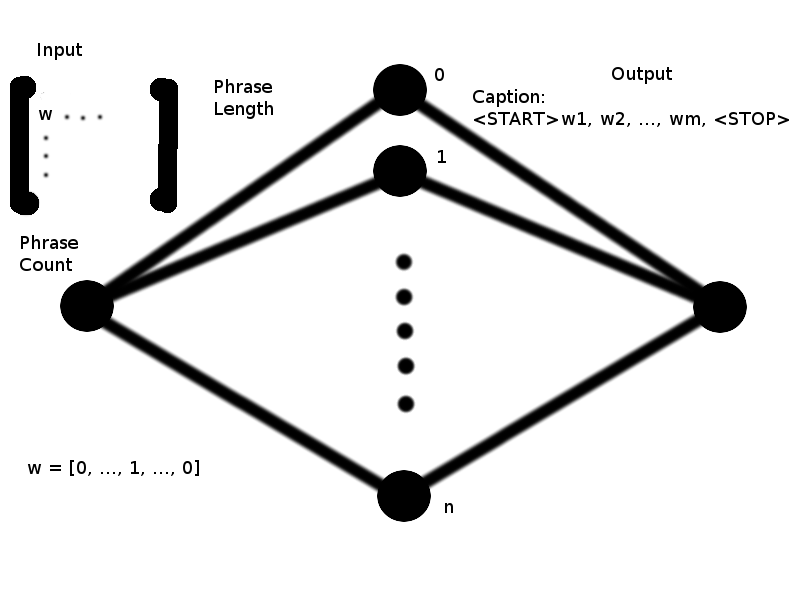
\includegraphics[width=8cm]{Untitled}
\caption{Current architecture}
\end{figure}
\end{document}
